\paragraph{GCMP}

The \gls{gcmp} is a more efficient alternative to \gls{ccmp} introduced in the \gls{ieee} 802.11ac amendment to allow devices to transfer data at higher speeds with less processing requirements \cite{ieee_80211_2020}. Just like \gls{ccmp}, it has a 128-bit (\gls{gcmp}-128) and a 256-bit (\gls{gcmp}-256) variants. \gls{wpa}3 enforces use of \gls{gcmp}-256 on \gls{wpa}3-Enterprise networks.

\begin{figure}[h]
    \centering
    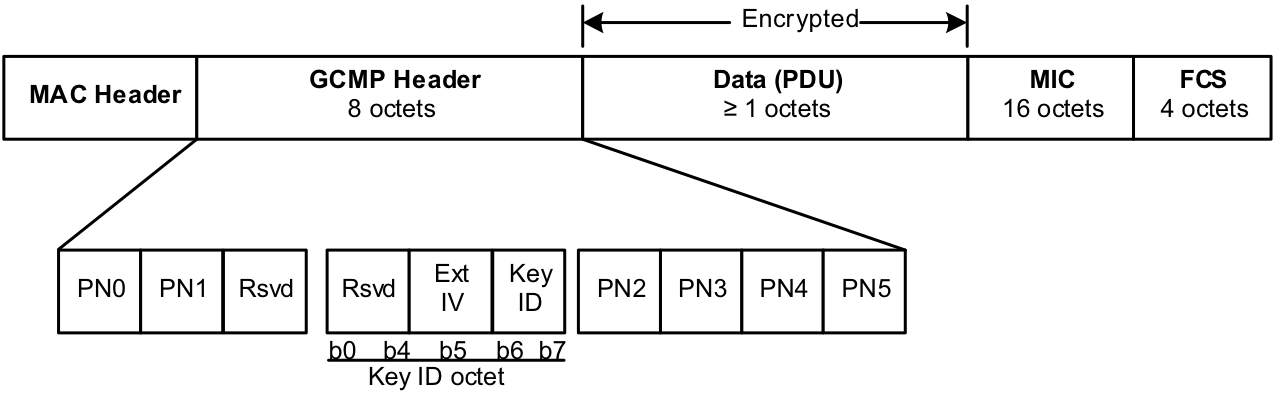
\includegraphics[width=\linewidth]{contents/background-in-wireless-networks/protected-network-standards/wpa3/gcmp/expanded-gcmp-mpdu.png}
    \caption{Expanded \gls{gcmp} \gls{mpdu}}
    {Source: \cite{ieee_80211_2020}}
    \label{figure:ieee80211_figure1226}
\end{figure}

Represented by Figure \ref{figure:ieee80211_figure1226}, the \gls{mpdu} of \gls{gcmp} is very similar to the \gls{ccmp} one, the \gls{mic} size being the only difference between them. Instead of a variant \gls{mic} size for 128-bit and 256-bit keys, \gls{gcmp}’s \gls{mic} is always 16-octet long.

\begin{figure}[h]
    \centering
    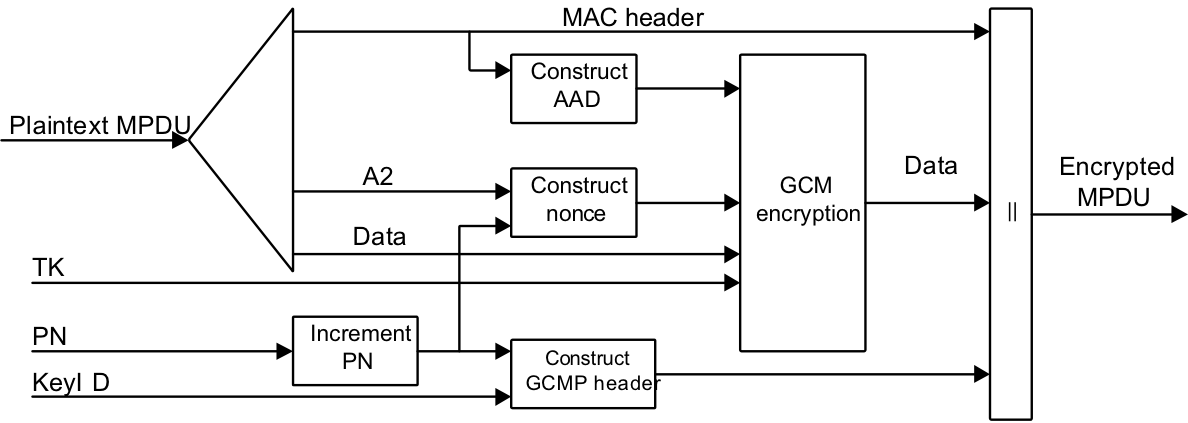
\includegraphics[width=\linewidth]{contents/background-in-wireless-networks/protected-network-standards/wpa3/gcmp/gcmp-encapsulation-block-diagram.png}
    \caption{\gls{gcmp} Encapsulation Block Diagram}
    {Source: \cite{ieee_80211_2020}}
    \label{figure:ieee80211_figure1227}
\end{figure}

The encapsulation process, shown on Figure \ref{figure:ieee80211_figure1227}, differs from \gls{ccmp} on the Nonce construction. The priority is no longer considered, only \gls{a2} and \gls{pn} still remain. As expected, the \gls{ccmp} Header construction is replaced with the \gls{gcmp} Header construction and the \gls{ccm} Originator Processing with the \gls{gcm} Originator Processing.

\begin{figure}[h]
    \centering
    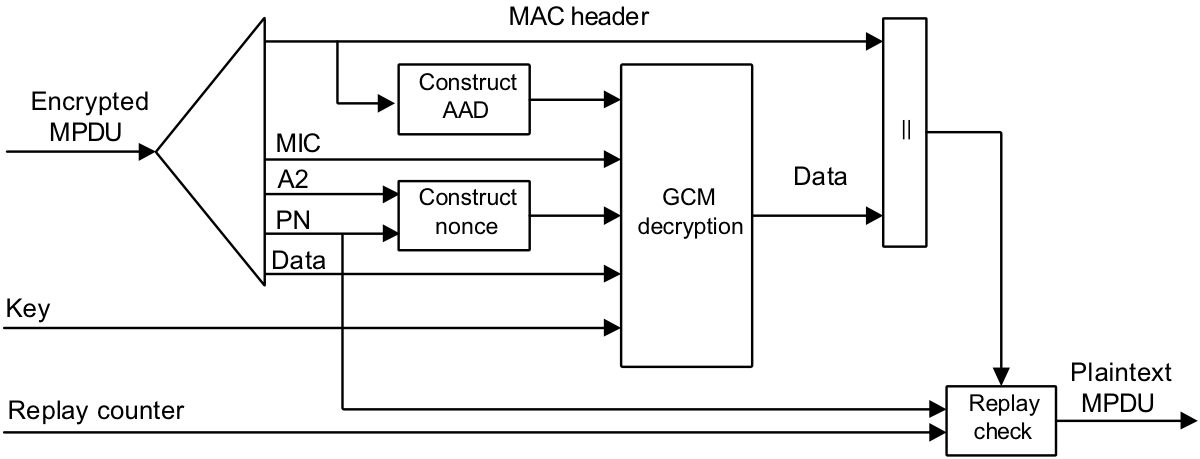
\includegraphics[width=\linewidth]{contents/background-in-wireless-networks/protected-network-standards/wpa3/gcmp/gcmp-decapsulation-block-diagram.png}
    \caption{\gls{gcmp} Decapsulation Block Diagram}
    {Source: \cite{ieee_80211_2020}}
    \label{figure:ieee80211_figure1229}
\end{figure}

On decapsulation, the \gls{ccm} Recipient Processing is substituted by the \gls{gcm} Recipient Processing. The Nonce construction is performed just like in the encapsulation process. The process is shown on Figure \ref{figure:ieee80211_figure1229}.

\FloatBarrier
